\label{chap:technology}

Chương này trình bày tổng quan các công nghệ được lựa chọn để xây dựng hệ thống, mô hình kiến trúc các tầng và luồng tương tác giữa chúng, đồng thời phân tích ưu nhược điểm và lý do lựa chọn. Nội dung bám theo sơ đồ kiến trúc tổng thể (Hình~\ref{fig:tech_architecture_overview}) và được điều chỉnh cho phù hợp với cách triển khai thực tế trên \textbf{máy chủ VPS}.

\section{Kiến trúc tổng thể và stack công nghệ}
\label{sec:tech_stack_overview}

Hình~\ref{fig:tech_architecture_overview} mô tả kiến trúc logic toàn hệ thống: người dùng truy cập qua web (máy tính hoặc trình duyệt trên di động), tầng Frontend (React/Vite) giao tiếp với Backend (Node.js/Express) bằng \textbf{HTTP/REST (JSON)} cho các thao tác nghiệp vụ và \textbf{WebSocket (Socket.IO)} cho tính năng thời gian thực (thông báo, tín hiệu tương tác). Backend kết nối \textbf{MongoDB} qua \textbf{Mongoose ODM}, lưu trữ và phân phối media qua \textbf{Cloudinary (CDN)}, đồng thời gọi các \textbf{API bên thứ ba} (bản đồ, LLM, OAuth).

\begin{itemize}
    \item \textbf{Frontend:} React 18, Vite, Tailwind CSS, DaisyUI, TanStack Query; \texttt{face-api.js} hỗ trợ xử lý nhận diện khuôn mặt / kiểm tra ảnh phía trình duyệt (phù hợp với lớp ``NSFW \& Face'' trên sơ đồ).
    \item \textbf{Giao tiếp mạng:} REST JSON; Socket.IO (WebSocket + polling) cho kênh hai chiều.
    \item \textbf{Backend:} Node.js, Express.js, TypeScript; xác thực \textbf{JWT}; đăng nhập \textbf{OAuth 2.0} (Google; sơ đồ minh họa thêm khả năng mở rộng Facebook/GitHub).
    \item \textbf{Nhóm nghiệp vụ trên API:} Auth, User, nội dung (bài viết, sự kiện, \ldots), kênh chat/thời gian thực, proxy AI (tương thích OpenAI API), xử lý ảnh liên quan kiểm duyệt/nhận diện.
    \item \textbf{Cơ sở dữ liệu:} MongoDB (sơ đồ minh họa MongoDB Atlas dạng replica set; triển khai có thể dùng Atlas hoặc MongoDB cài trên cùng/VPS khác).
    \item \textbf{Media:} Cloudinary (upload, biến đổi ảnh, CDN).
    \item \textbf{Tích hợp ngoài:} API LLM kiểu OpenAI (trong mã nguồn dùng endpoint tương thích OpenAI qua Groq); \textbf{Goong Maps API} (bản đồ, địa lý --- tương ứng nhóm ``Maps/Geocoding'' trên sơ đồ); OAuth Google.
\end{itemize}

\begin{figure}[H]
    \centering
    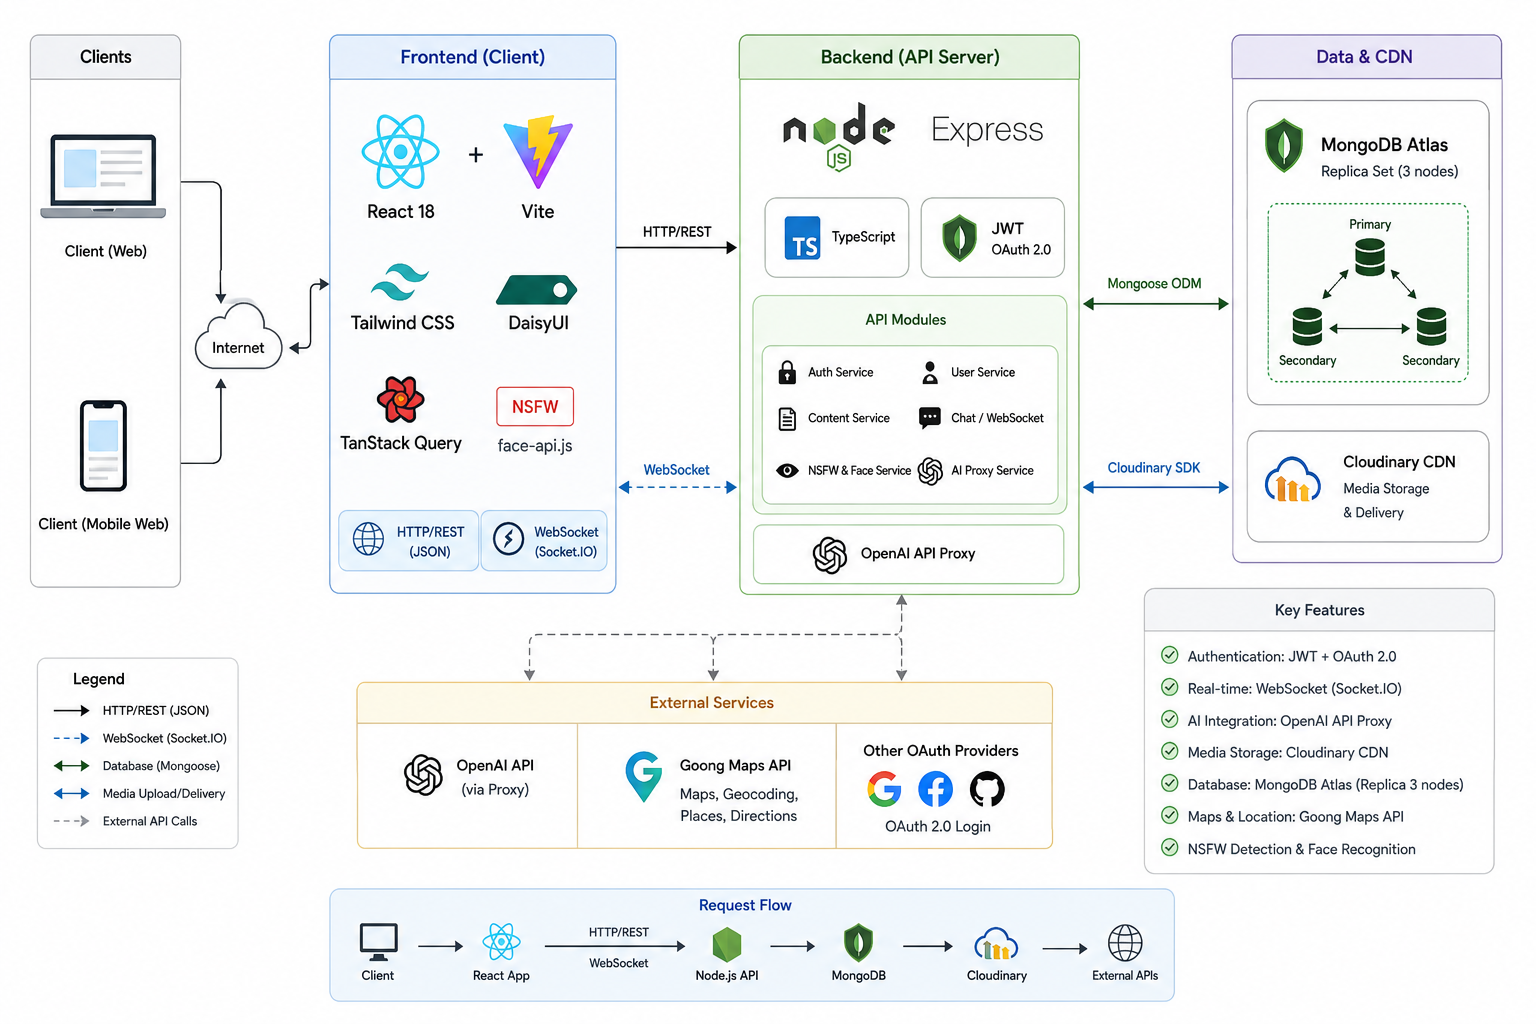
\includegraphics[width=\textwidth]{Images/IMG/Kientruchethong.png}
    \vspace{0.75em}
    \caption{Kiến trúc tổng thể hệ thống: client, Frontend (React/Vite), Backend (Node/Express), tầng dữ liệu (MongoDB, Cloudinary) và dịch vụ ngoài; chú thích luồng HTTP/REST, WebSocket, truy vấn CSDL và upload media.}
    \label{fig:tech_architecture_overview}
\end{figure}

Luồng xử lý điển hình (tham chiếu phần ``Request flow'' trên sơ đồ): \textbf{Client} $\rightarrow$ ứng dụng React $\rightarrow$ (HTTP và/hoặc WebSocket) $\rightarrow$ API Node.js $\rightarrow$ MongoDB và/hoặc Cloudinary $\rightarrow$ gọi API ngoài khi cần.

\section{Công nghệ Frontend và Backend}
\label{sec:tech_frontend}

Bảng~\ref{tab:tech_stack_detail} tóm tắt các công nghệ cốt lõi ở tầng Frontend và Backend, cùng lý do lựa chọn.

\begin{table}[H]
\centering
\caption{Công nghệ Frontend và Backend}
\label{tab:tech_stack_detail}
\small
\renewcommand{\arraystretch}{1.2}
\begin{tabular}{|p{3.2cm}|p{2.5cm}|p{8.3cm}|}
\hline
\textbf{Công nghệ} & \textbf{Lĩnh vực} & \textbf{Mục đích \& Lý do lựa chọn} \\
\hline
\textbf{React.js 18} \cite{ReactJSDocs} & Frontend UI & SPA theo component, hiệu năng tốt; hệ sinh thái TanStack Query, React Hook Form, React Router. \\
\hline
\textbf{TypeScript} \cite{TypeScriptDocs} & Backend (và có thể mở rộng FE) & Kiểu tĩnh, an toàn kiểu, bảo trì dài hạn; Backend hiện thực bằng TypeScript. \\
\hline
\textbf{Tailwind CSS + DaisyUI} & Frontend Styling & Utility-first, bundle gọn, responsive; DaisyUI thống nhất giao diện. \\
\hline
\textbf{Vite} & Build Tool & Khởi động nhanh, HMR, tối ưu bundle production. \\
\hline
\textbf{Node.js + Express.js} \cite{NodeJSDocs,ExpressJSDocs} & Backend API & I/O bất đồng bộ, một ngôn ngữ với Frontend; middleware linh hoạt; tích hợp Socket.IO trên cùng máy chủ HTTP. \\
\hline
\textbf{Socket.IO} & Frontend + Backend & Trừu tượng hóa WebSocket, fallback polling, phù hợp thông báo và tín hiệu thời gian thực. \\
\hline
\end{tabular}
\end{table}

\begin{figure}[H]
   \centering
   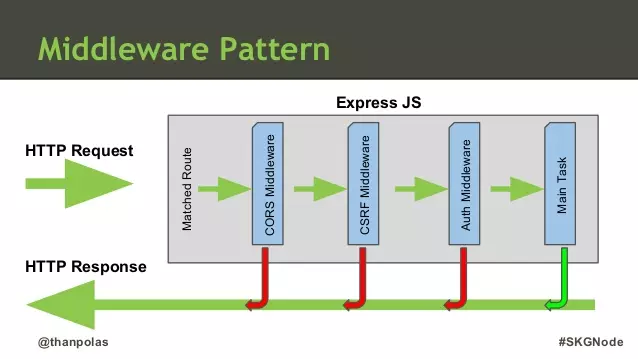
\includegraphics[width=0.65\textwidth]{Images/Middleware.png}
   \vspace{1em}
   \caption{Luồng xử lý request với middleware trong Express.js \cite{VibloMiddleware}}
   \label{fig:expressjs_middleware}
\end{figure}

\section{Cơ sở dữ liệu và dịch vụ bổ trợ}
\label{sec:tech_database}

\subsection{MongoDB và Cloudinary}
\label{subsec:tech_mongodb}

\textbf{MongoDB} \cite{MongoDBDocs} là CSDL NoSQL hướng tài liệu (BSON), phù hợp dữ liệu đa dạng của mạng xã hội thể thao. Mongoose ODM cung cấp schema, validation và truy vấn có cấu trúc. Trên sơ đồ, cụm MongoDB Atlas (replica set) thể hiện mô hình vận hành khuyến nghị khi dùng dịch vụ quản lý; khi tự host trên VPS vẫn giữ cùng vai trò logic trong kiến trúc.

\textbf{Cloudinary} là dịch vụ lưu trữ và phân phối media qua CDN; Backend tích hợp SDK để upload, nhận URL an toàn (HTTPS), giảm tải lưu trữ tĩnh trên VPS.

\begin{figure}[H]
   \centering
   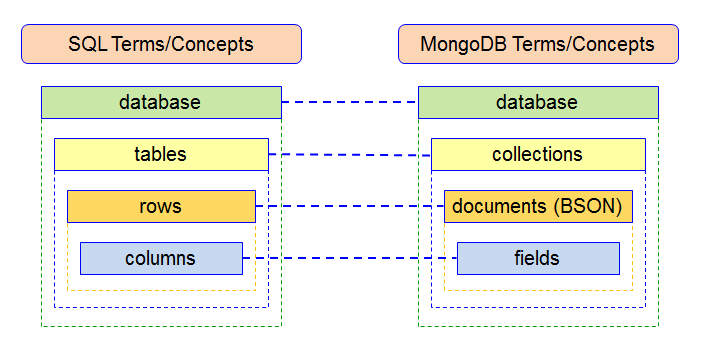
\includegraphics[width=0.65\textwidth]{Images/MongodbandSQL.png}
   \vspace{1em}
   \caption{So sánh cấu trúc dữ liệu MongoDB và SQL}
   \label{fig:mongodb_vs_sql}
\end{figure}

\subsection{Công nghệ triển khai: máy chủ VPS}
\label{subsec:tech_deployment_analysis}

Hệ thống được triển khai trên \textbf{máy chủ VPS} chạy \textbf{Ubuntu}: một máy ảo thuê riêng, tập trung toàn bộ tầng phục vụ ứng dụng (Nginx, tiến trình Node, tùy chọn MongoDB cục bộ). Sơ đồ Hình~\ref{fig:tech_architecture_overview} mô tả \textbf{kiến trúc logic} (thành phần và luồng nghiệp vụ); Hình~\ref{fig:vps_deployment} mô tả \textbf{sơ đồ triển khai VPS}---cách các thành phần đó được bố trí trên một host và điểm ra/vào qua Internet.

\begin{figure}[H]
    \centering
    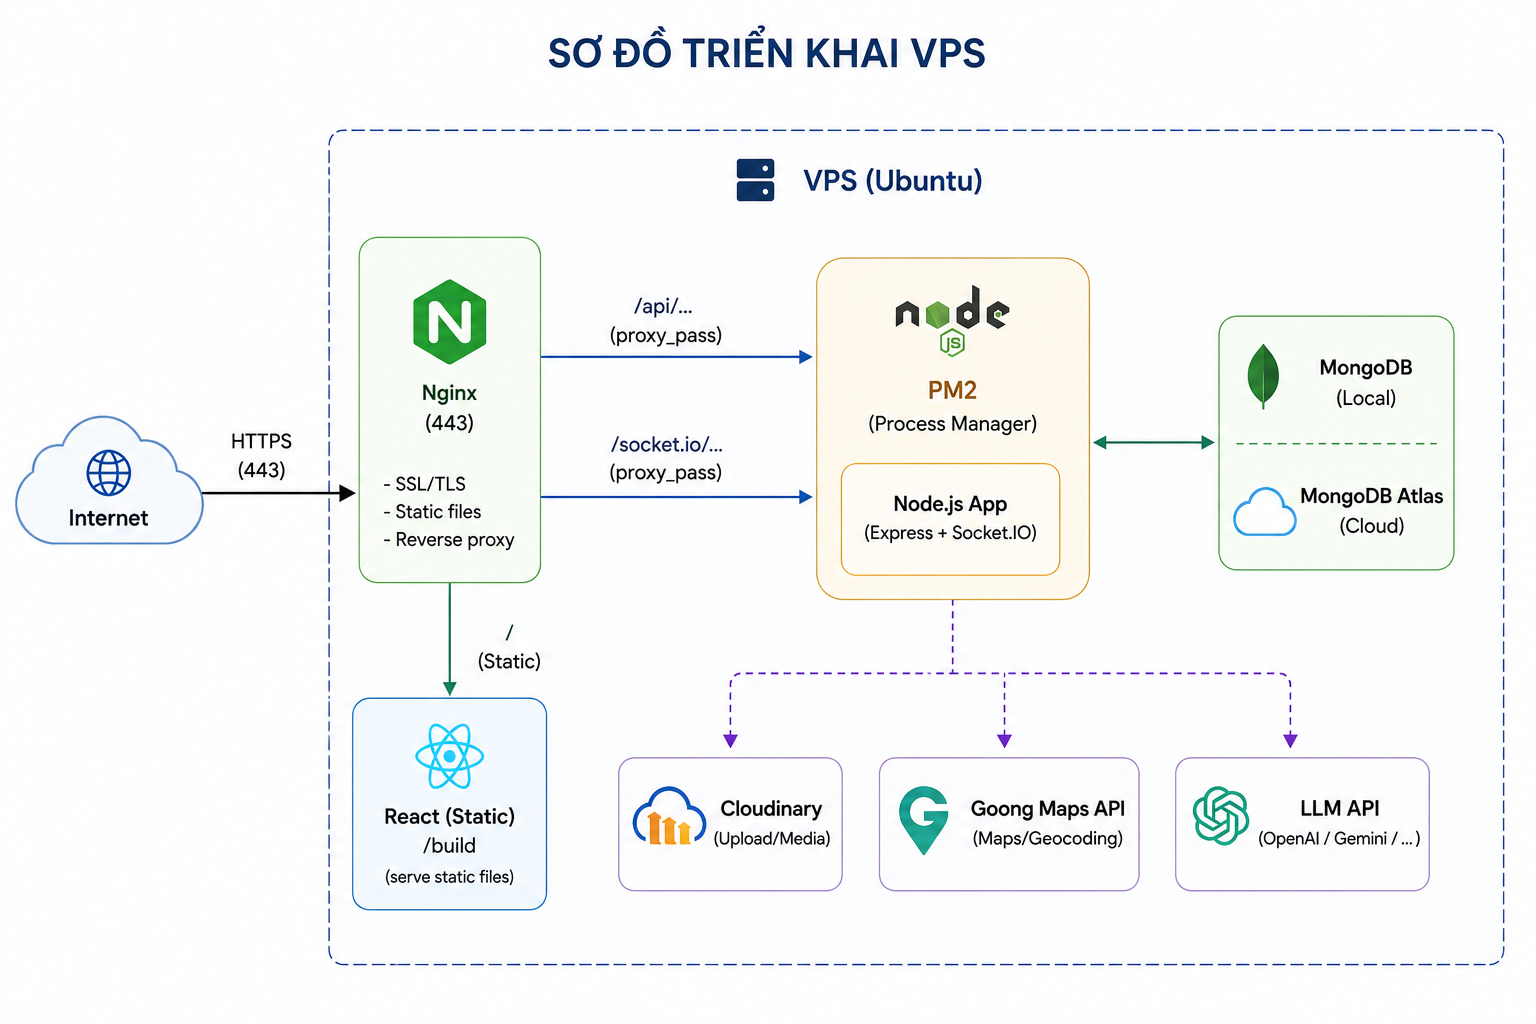
\includegraphics[width=\textwidth]{Images/IMG/deploy.png}
    \vspace{0.75em}
    \caption{Sơ đồ triển khai VPS: truy cập HTTPS, Nginx (TLS, static React, reverse proxy), ứng dụng Node.js (PM2, Express, Socket.IO), MongoDB (local hoặc Atlas), và tích hợp Cloudinary, Goong Maps, API LLM.}
    \label{fig:vps_deployment}
\end{figure}

\subsubsection{Luồng truy cập từ Internet}
Người dùng kết nối qua \textbf{Internet} tới địa chỉ public của VPS. Toàn bộ giao tiếp trình duyệt--máy chủ nên dùng \textbf{HTTPS (cổng 443)}: Nginx chấm dứt TLS (SSL/TLS), phát hành chứng chỉ ví dụ qua Let's Encrypt hoặc chứng chỉ thương mại. HTTPS là cần thiết cho OAuth, bảo vệ token JWT và cookie phiên.

\subsubsection{Nginx: reverse proxy và phục vụ tĩnh}
\textbf{Nginx} đóng vai trò điểm vào duy nhất (\textit{edge}) trước ứng dụng:
\begin{itemize}
    \item \textbf{SSL/TLS:} giải mã HTTPS, có thể bật HTTP/2, header bảo mật cơ bản.
    \item \textbf{React (tĩnh):} thư mục kết quả \texttt{npm run build} của Vite/React được cấu hình làm \textit{root} cho đường dẫn gốc \texttt{/}; Nginx phục vụ HTML/CSS/JS tĩnh, hiệu năng tốt và giảm tải cho Node.
    \item \textbf{Reverse proxy tới Node:} các yêu cầu có tiền tố \texttt{/api/...} được chuyển tiếp tới tiến trình Backend (REST JSON). Các yêu cầu \texttt{/socket.io/...} (và nâng cấp WebSocket tương thích Socket.IO) cũng được proxy tới cùng ứng dụng Node để thông báo, phòng gọi video và tín hiệu thời gian thực hoạt động đúng sau một cổng/domain thống nhất.
\end{itemize}
Cấu hình \texttt{proxy\_http\_version 1.1}, \texttt{Upgrade}, \texttt{Connection} cho đoạn WebSocket là thông lệ khi ghép Nginx với Socket.IO.

\subsubsection{Backend: Node.js, Express, Socket.IO và PM2}
Ứng dụng \textbf{Node.js} (Express, TypeScript sau biên dịch) lắng nghe cổng nội bộ (ví dụ \texttt{127.0.0.1:4000}), không expose trực tiếp ra Internet. \textbf{PM2} (hoặc \textbf{systemd}) giữ tiến trình sống, tự khởi động lại khi crash hoặc khi reboot VPS, ghi log tập trung---phù hợp vận hành production trên một máy. Một tiến trình duy nhất phục vụ cả REST và Socket.IO trên cùng HTTP server (mô hình MERN-style đã dùng trong dự án).

\subsubsection{Cơ sở dữ liệu trên VPS hoặc cloud}
Sơ đồ thể hiện hai hướng tương thích:
\begin{itemize}
    \item \textbf{MongoDB (local):} cài trực tiếp trên VPS, giảm độ trễ nội bộ và chi phí cluster; cần sao lưu, cập nhật bản vá và giới hạn tài nguyên RAM/đĩa.
    \item \textbf{MongoDB Atlas:} CSDL trên đám mây, VPS chỉ chạy ứng dụng; phù hợp khi muốn replica, backup và bảo trì do nhà cung cấp đảm nhiệm.
\end{itemize}
Ứng dụng chỉ cần chuỗi kết nối \texttt{MONGODB\_URL} phù hợp; Mongoose giữ nguyên vai trò ODM trong cả hai trường hợp.

\subsubsection{Dịch vụ bên thứ ba (ngoài VPS)}
Backend gọi ra Internet tới các API không nằm trên VPS:
\begin{itemize}
    \item \textbf{Cloudinary}---upload, lưu trữ và CDN cho ảnh/video.
    \item \textbf{Goong Maps API}---bản đồ, địa lý, tuyến đường (phía client dùng SDK/map tiles; server có thể dùng khi cần).
    \item \textbf{LLM API}---các nhà cung cấp như OpenAI, Gemini hoặc endpoint tương thích OpenAI (trong mã nguồn hiện tại có tích hợp kiểu OpenAI-compatible, ví dụ Groq) cho tính năng gợi ý, kiểm tra nội dung, v.v.
\end{itemize}
Các khóa API được đặt trong biến môi trường trên VPS, không đưa vào mã nguồn.

\subsubsection{Tùy chọn: Docker và email AWS SES}
\textbf{Docker} \cite{DockerDocs} (Hình~\ref{fig:docker_architecture}) có thể đóng gói Backend hoặc toàn stack để đồng nhất môi trường; trên VPS production vẫn thường cần Nginx phía trước container (hoặc tương đương) cho TLS và tĩnh. \textbf{AWS SES} có thể dùng để gửi email hệ thống, độc lập với việc ứng dụng chạy trên VPS (không bắt buộc EC2/CloudFront).

\begin{figure}[H]
   \centering
   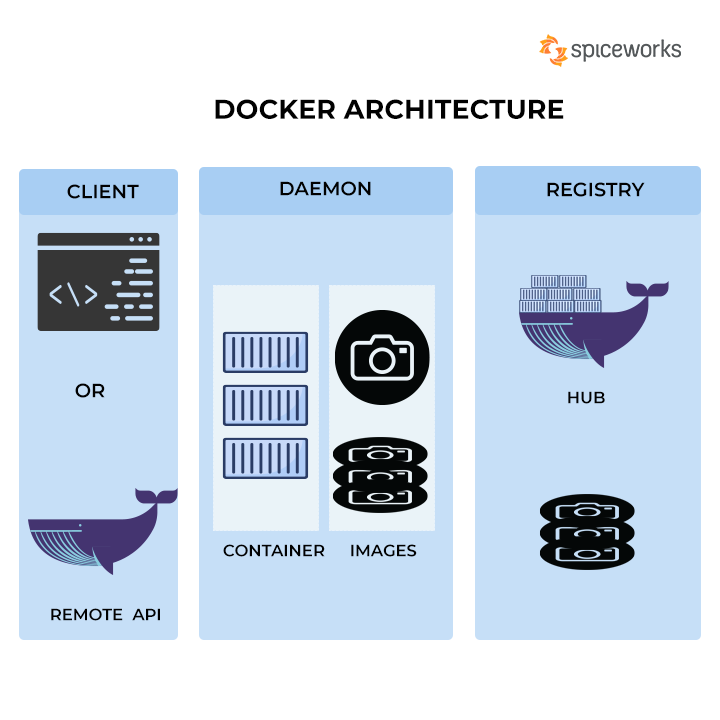
\includegraphics[width=0.7\textwidth]{Images/Docker-Architecture.png}
   \vspace{1em}
   \caption{Kiến trúc Docker \cite{DockerDocs} (công cụ đóng gói tùy chọn khi triển khai)}
   \label{fig:docker_architecture}
\end{figure}

\section{Kết luận}
\label{sec:tech_conclusion}

Stack và kiến trúc được chọn theo các tiêu chí: đáp ứng chức năng mạng xã hội thể thao, hiệu năng tốt, khả năng mở rộng, cộng đồng lớn và tốc độ phát triển. React + Vite + Tailwind/DaisyUI xây dựng giao diện hiện đại; Node.js + Express + TypeScript phục vụ REST và Socket.IO; MongoDB + Mongoose lưu trữ linh hoạt; Cloudinary đảm nhiệm media; tích hợp LLM (API kiểu OpenAI), Goong Maps và OAuth bổ sung năng lực thông minh và bản đồ. Triển khai thực tế trên \textbf{VPS Ubuntu} (Hình~\ref{fig:vps_deployment}) dùng Nginx (HTTPS, static build, proxy \texttt{/api} và \texttt{/socket.io}), PM2 cho Node, MongoDB local hoặc Atlas, và các API ngoài cho media, bản đồ và LLM. Thiết kế chi tiết use case và thành phần hệ thống được trình bày tại Chương~\ref{chap:system_design}.

\textbf{Hướng phát triển:} Redis cache, hàng đợi message, CI/CD, giám sát (Prometheus/Grafana), mở rộng đa máy chủ hoặc tách tier khi tải tăng.
